\documentclass{scrartcl}\usepackage[]{graphicx}\usepackage[]{color}
%% maxwidth is the original width if it is less than linewidth
%% otherwise use linewidth (to make sure the graphics do not exceed the margin)
\makeatletter
\def\maxwidth{ %
  \ifdim\Gin@nat@width>\linewidth
    \linewidth
  \else
    \Gin@nat@width
  \fi
}
\makeatother

\definecolor{fgcolor}{rgb}{0.345, 0.345, 0.345}
\newcommand{\hlnum}[1]{\textcolor[rgb]{0.686,0.059,0.569}{#1}}%
\newcommand{\hlstr}[1]{\textcolor[rgb]{0.192,0.494,0.8}{#1}}%
\newcommand{\hlcom}[1]{\textcolor[rgb]{0.678,0.584,0.686}{\textit{#1}}}%
\newcommand{\hlopt}[1]{\textcolor[rgb]{0,0,0}{#1}}%
\newcommand{\hlstd}[1]{\textcolor[rgb]{0.345,0.345,0.345}{#1}}%
\newcommand{\hlkwa}[1]{\textcolor[rgb]{0.161,0.373,0.58}{\textbf{#1}}}%
\newcommand{\hlkwb}[1]{\textcolor[rgb]{0.69,0.353,0.396}{#1}}%
\newcommand{\hlkwc}[1]{\textcolor[rgb]{0.333,0.667,0.333}{#1}}%
\newcommand{\hlkwd}[1]{\textcolor[rgb]{0.737,0.353,0.396}{\textbf{#1}}}%

\usepackage{framed}
\makeatletter
\newenvironment{kframe}{%
 \def\at@end@of@kframe{}%
 \ifinner\ifhmode%
  \def\at@end@of@kframe{\end{minipage}}%
  \begin{minipage}{\columnwidth}%
 \fi\fi%
 \def\FrameCommand##1{\hskip\@totalleftmargin \hskip-\fboxsep
 \colorbox{shadecolor}{##1}\hskip-\fboxsep
     % There is no \\@totalrightmargin, so:
     \hskip-\linewidth \hskip-\@totalleftmargin \hskip\columnwidth}%
 \MakeFramed {\advance\hsize-\width
   \@totalleftmargin\z@ \linewidth\hsize
   \@setminipage}}%
 {\par\unskip\endMakeFramed%
 \at@end@of@kframe}
\makeatother

\definecolor{shadecolor}{rgb}{.97, .97, .97}
\definecolor{messagecolor}{rgb}{0, 0, 0}
\definecolor{warningcolor}{rgb}{1, 0, 1}
\definecolor{errorcolor}{rgb}{1, 0, 0}
\newenvironment{knitrout}{}{} % an empty environment to be redefined in TeX

\usepackage{alltt}

\usepackage[utf8]{inputenc}
\usepackage{graphicx}%GRaphiken
\usepackage{tabularx}%Tabellen!
\usepackage[english]{babel}% Zeilentrennung besser
\usepackage{url}% Urls besser
\usepackage{textcomp}% Sonderzeichen
\usepackage{amsmath}%maths / equations
\usepackage{helvet}% Schrift Helvetica
% \usepackage[helvet]{sfmath}% Helvet also in Math modes
% \renewcommand\familydefault{\sfdefault}
\usepackage{sansmath} % sans in math
\usepackage[
	left=3cm,
	right=2cm,
	top=1.5cm,
	bottom=1cm
	,
	includeheadfoot
	]{geometry}														% Satzspiegel
\usepackage[
	round,	%(defaultage in the main file and \input ) for round parentheses;
	%square,	% for square brackets;
	%curly,	% for curly braces;
	%angle,	% for angle brackets;
	colon,	% (default) to separate multiple citations with colons;
	%comma,	% to use commas as separaters;
	authoryear,% (default) for author-year citations;
	%numbers,	% for numerical citations;
	%super,	% for superscripted numerical citations, as in Nature;
	sort,		% orders multiple citations into the sequence in which they appear in the list of 				references;
	%sort&compress,    % as sort but in addition multiple numerical citations
                   % are compressed if possible (as 3-6, 15);
	%longnamesfirst,  % makes the first citation of any reference the equivalent of
                   % the starred variant (full author list) and subsequent citations
                   %normal (abbreviated list);
	%sectionbib,      % redefines \thebibliography to issue \section* instead of \chapter*;
                   % valid only for classes with a \chapter command;
                   % to be used with the chapterbib package;
	%nonamebreak,     % keeps all the authors names in a citation on one line;
                   %causes overfull hboxes but helps with some hyperref problems.
]{natbib}											    			% Literaturverzeichnis
\usepackage{scrhack}   % kills \float@addtolists!  warning
\usepackage[pdfpagelabels,plainpages=false, pageanchor=false]{hyperref}	


%% andere Einstellungen
\linespread{1.5}% 1.5 Zeilenabstand			
\graphicspath{{fig/}}                     % path to graphics

\title{Use the GLM, Luke.}
\subtitle{How the use of proper statistical models can increase statistical power in ecotoxicological experiments.}
\author{Eduard Szöcs}
\date{\today}
\IfFileExists{upquote.sty}{\usepackage{upquote}}{}
\begin{document}
\maketitle

\section{Introduction}
Not mentioned in Newman (2013). 

Sparsely in OECD Guideline. 

Canada: 'The concept is quite advanced and as yet is not widely used in environmental toxicology.'

Wang/Riffel vergleichen NP aber kein Wort über GLM.

Brock et al. empfiehlt das sampling zui verbessern um die MDD zu verkleinern, keine erwähnung von GLMs (damit erhöhen die auch die power, wie man sieht und sind kostenlos)


Schon oft angesprochen (O'Hara 2010, Warton 2010 (arcsine is asinine), ?), aber nicht in der Ökotox aufgenommen.

MDD eigentlich nur ein synonym für power.

Obwohl jeder weiß dass NOEC blöd sind - werden sie weiter genutzt (siehe zb. viele publicationen von Fox). Fox 2012: "A
recurring concern expressed about the suggested move to
model-based inference is that the derived toxicity measure
will be influenced by a host of subjective decisions such as the
choice of the mathematical model, its parameterization, and
the estimation strategy."

Hoenig and Heisey: No post-hoc power estimation. Equally unhelpful are
post hoc estimates of minimum significant difference or de-
tectable ES. Once we have constructed a con-
fidence interval, power calculations yield no additional in-
sights’


\subsection{Transformation + Normal Model}
\begin{align}
  log(Ay_i + 1) \sim N(\mu_i, \sigma^2) \nonumber \\
  log(Ay_i + 1) = \alpha + \beta x_i \nonumber \\
  var(log(Ay_i + 1)) = \sigma^2 \label{eqn:1}
\end{align}


\subsection{Generalized Linear Model}
\begin{align}
  y_i \sim NB(\mu_i, \theta)  \nonumber \\
  log(\mu_i) = \alpha + \beta x_i   \nonumber \\
  var(y_i) = \mu_i + \mu_i^2 / \theta  \label{eqn:2}
\end{align}


\section{Methods}

Literature review of SETAC Journals -> NOEC, GLM, log/arcsine transformation? How often, what is applied?



\subsection{Simulation scenarios}
We simulated data that mimics count data encountered in mesocosm experiments, with five treatments (T1-T5) and one control (C). 
Mean abundance in treatments T2-T5 was reduced to half of the control treatment and T1 ($\mu_\text{\tiny T2} = ... = \mu_\text{\tiny T5} = 0.5 \mu_\text{\tiny C} = 0.5 \mu_\text{\tiny T1} $). Therefore, the theoretical LOEC is at T2 and the NOEC correspondingly at T1.
Counts were drawn from a negative binomial distribution with a fixed $\theta = 3.91$ for all treatments.

We simulated datasets with different the number of replicates (N = \{3, 6, 9, 12\}) and different abundances in control treatments ($\mu_\text{\tiny C}$ = \{2, 4, 8, 16, 32, 64, 128, 256, 512, 1024 \}). For each combination we generated 100 datasets.

Each dataset was analysed with different methods/models.

\subsubsection{Global test of treatment effect}
2 different models were fitted to the data. 
A model assuming a normal distribution after ln(Ay + 1) transforming the response (eqn \ref{eqn:1}) and a model assuming that the response follows a negative binomial distribution.
Treatment effects were in both cases investigated using a Likelihood-Ratio-Test.
Moreover, we applied a non-parametric Kruskal-Wallis Rank Sum Test.

1) POWER = ability to detect an effect that is present.
their accuracy at
2) (Type I error) : maintaining a significance level of 0.05 when there is no
effect to be detected. Maybe check also this.

\subsubsection{Determination of LOEC/NOEC}
multcomp, nparcomp, pairwise-wilcox.
Check p-value adjustment between methods!

Add untransformed





Derzeit, muT = 1/2 muC. Deshalb nimmt die power ab mit kleiner muC (die differnz wird kleiner). Wie kann man das umgehen/besser machen?

Andere Daten/Szenarios? Siehe Wang oder Newman.

\begin{figure}
  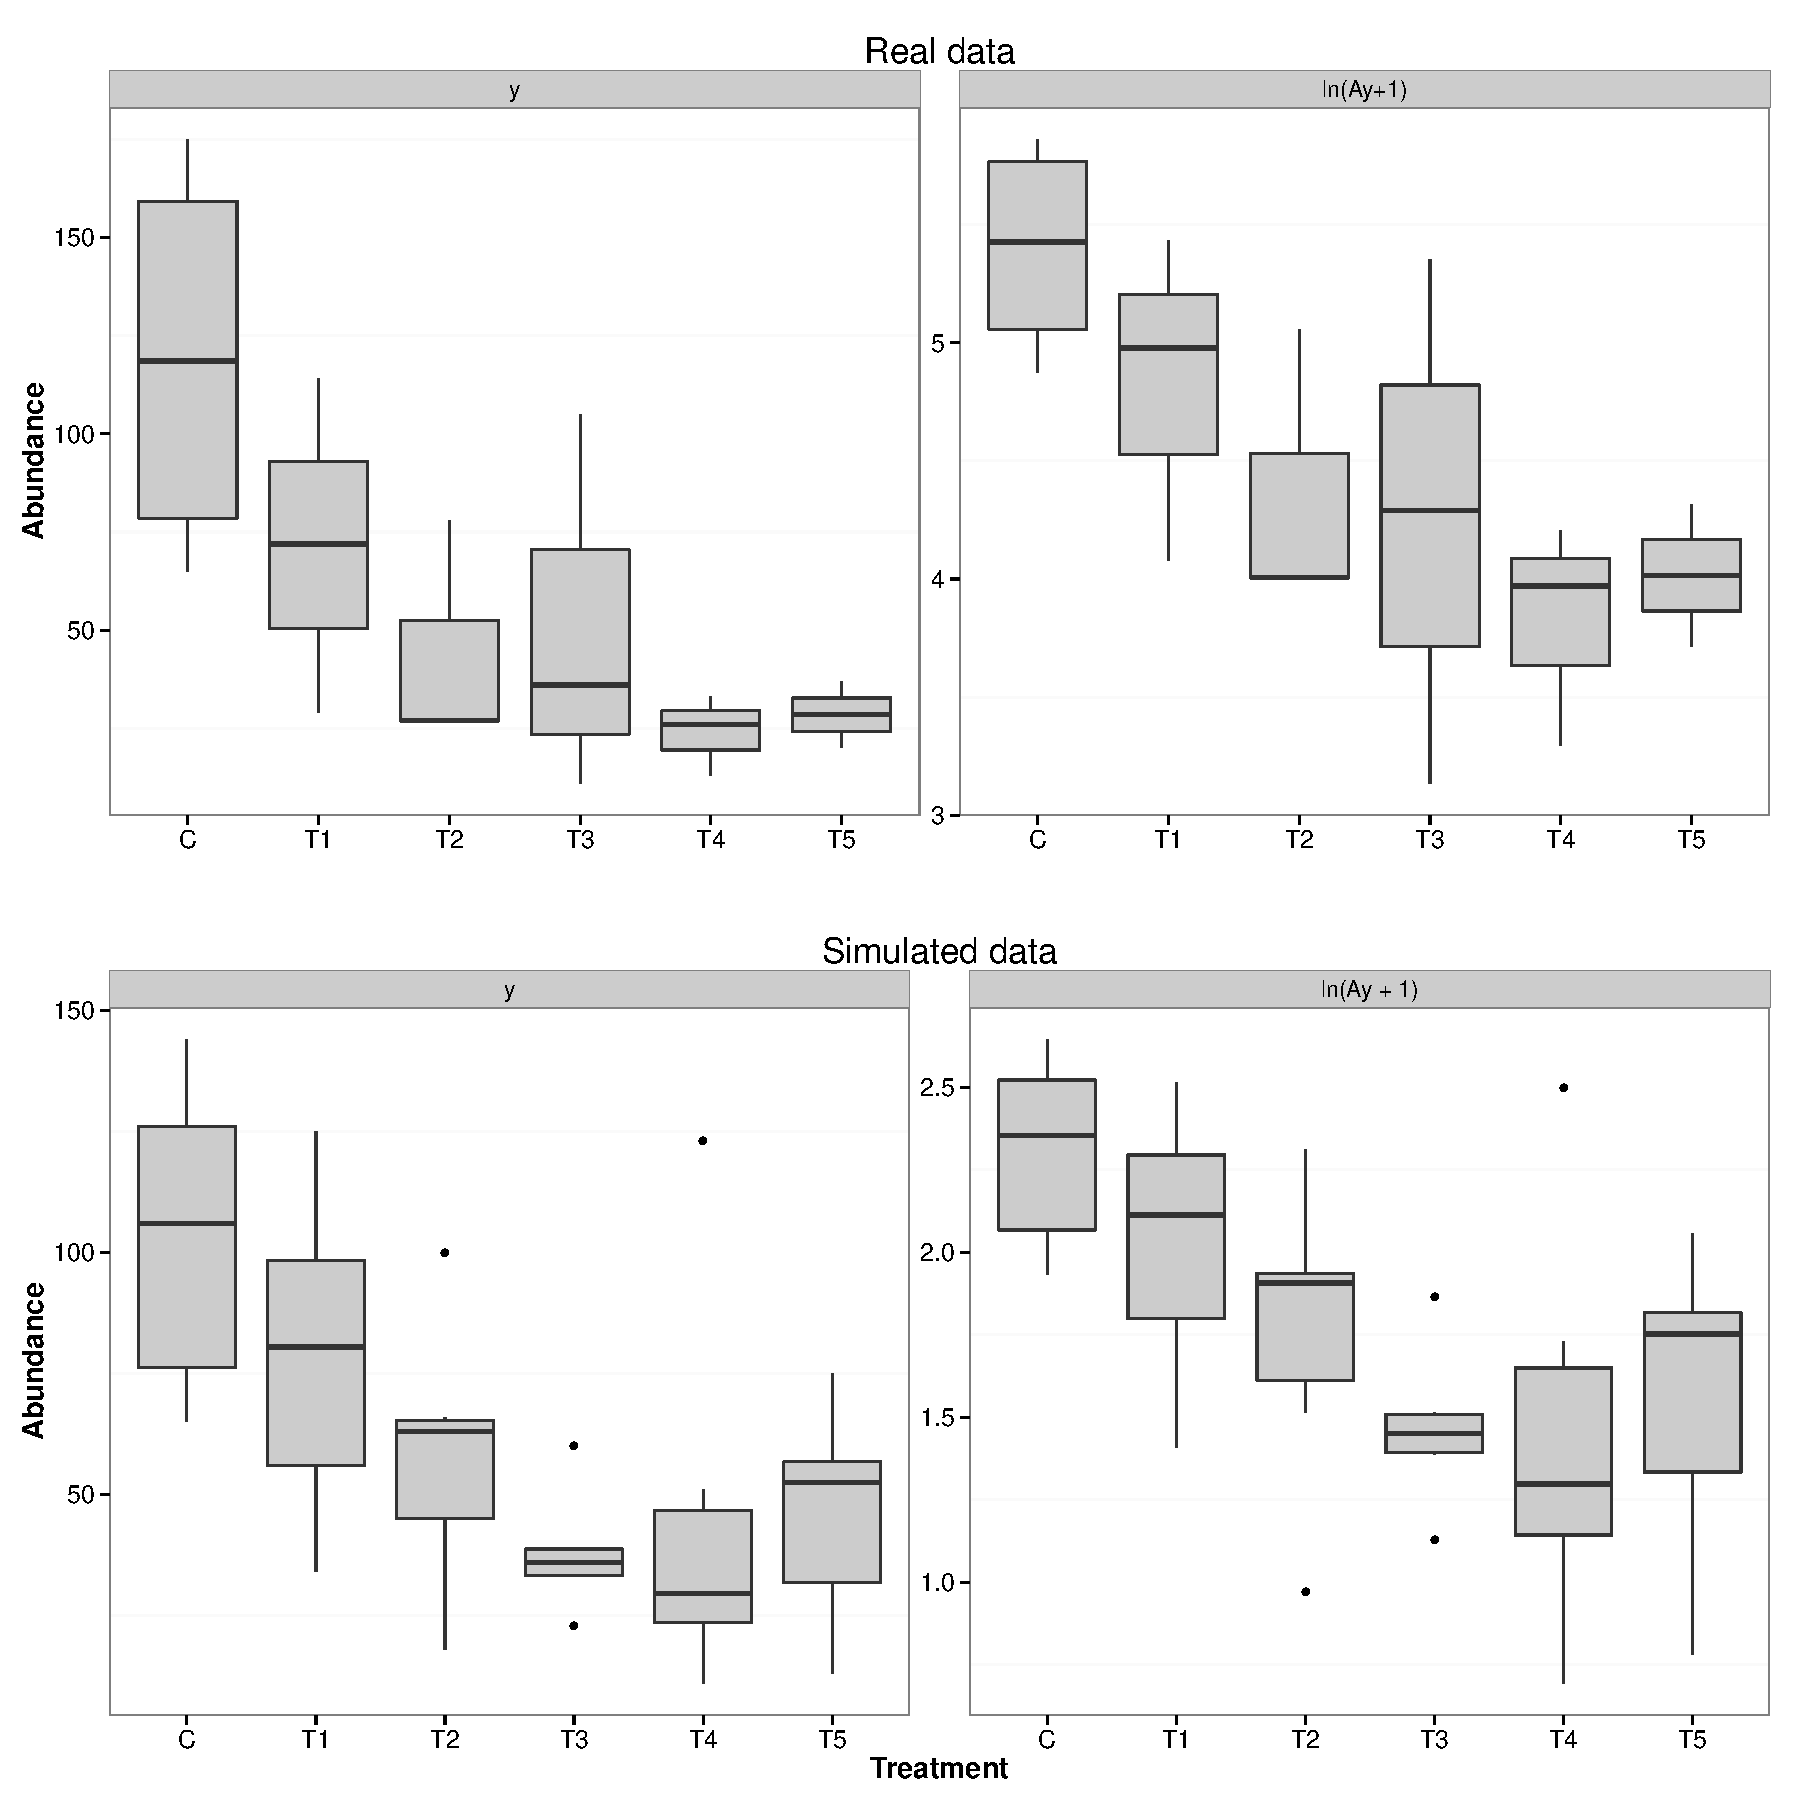
\includegraphics[width = \textwidth]{p4_1.pdf}
  \caption{Real data from Brock et al... (top) and one realisation of simulated data (below, N = 6, $\mu_c$ = 100). Left panel show raw counts, right panel $log(A \cdot x + 1)$ transformed counts.}
  \label{fig:p4_1}
\end{figure}

% \subsection{Simulations based on real data}
% Or real data (no simulation) - because post-hoc power is crap?
% Brock et al data.
% Different species of chlorpyrifos.
% -> densities proportions etc wäre noch cool.... Wang/Riffel?
% Newman: Example 5.1 for arcsine


\section{Results}
\subsection{Simulation scenarious}

\begin{figure}
  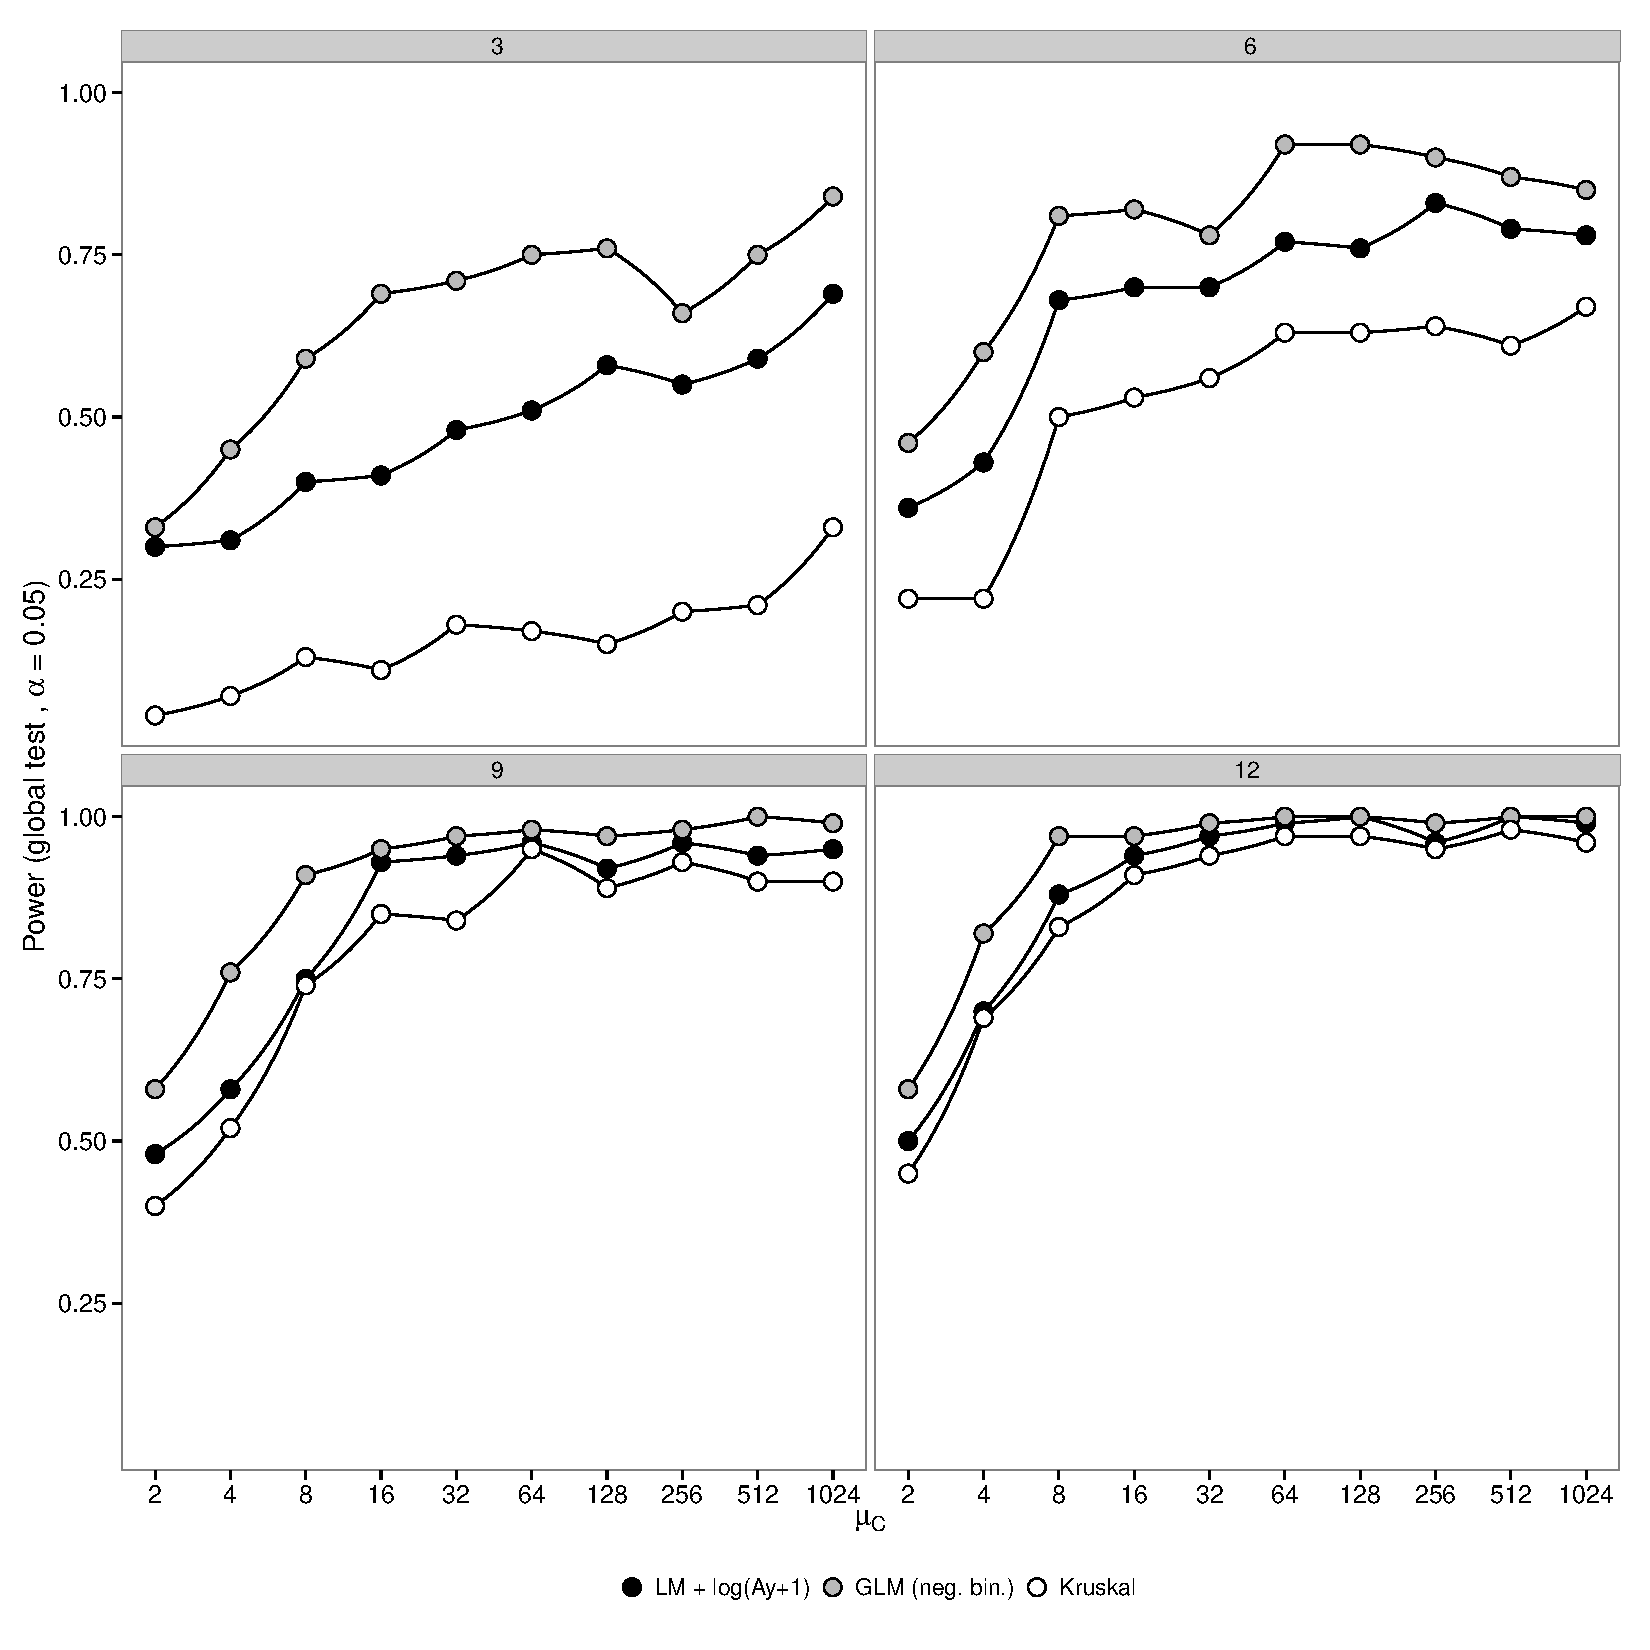
\includegraphics[width = \textwidth]{p2.pdf}
  \caption{Power.}
  \label{fig:p2}
\end{figure}

\begin{figure}
  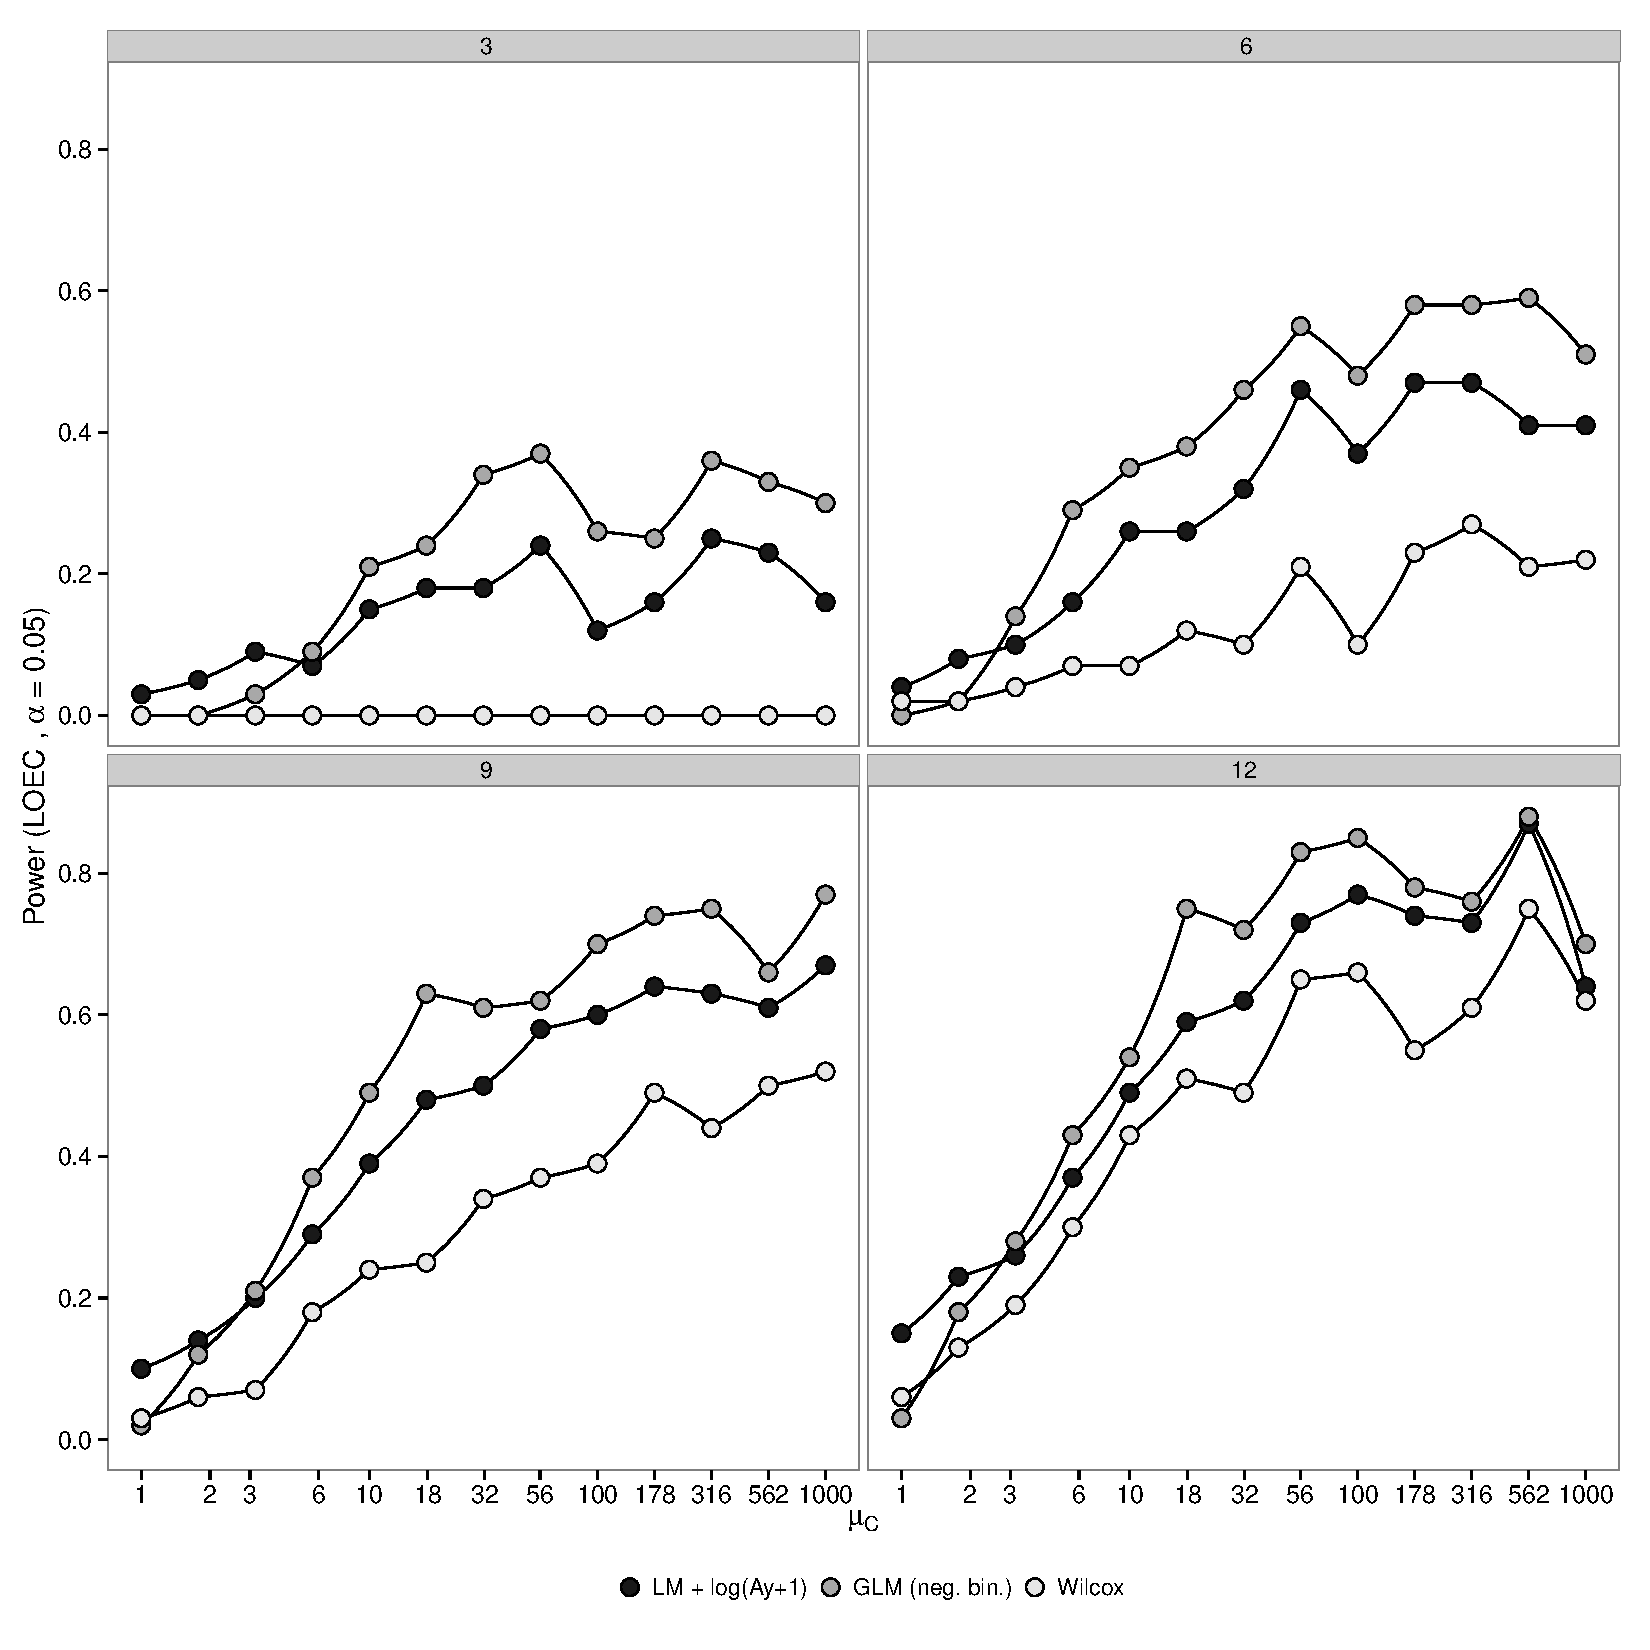
\includegraphics[width = \textwidth]{p3.pdf}
  \caption{Power to detect LOEC.}
  \label{fig:p3}
\end{figure}

-> bei kleinerm muc lm besser weil annahmen nicht passen (checken)?

% \subsection{Simulations based on real data}

\section{Discussion}

Decide between NB and P? - Mean-Var-Plot!

\section{Conclusion}

\appendix
\section{Tipps
(Or move up to introduction?)
Check distribution}


\section{TODO}
Read about nparcomp.




\end{document}
